
\documentclass[11pt]{article}
\usepackage{jeffe,handout}
\usepackage{tikz}
\usepackage{pgfkeys}
\usetikzlibrary{positioning,chains,fit,shapes,calc,graphs}

\usepackage{multicol}
\newcommand{\marksamt}[1]{\textbf{[#1~marks]}}
\newcommand{\markamt}[1]{\textbf{[#1~mark]}}
\newcommand{\answerMC}[1]{
\begin{tikzpicture}\draw[black, fill=black] circle [radius=0.35em];\end{tikzpicture}\ #1}
\newcommand{\fillinMC}[1]{\fillinMCmath{\mbox{#1}}}
\newcommand{\fillinMCmath}[1]{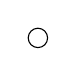
\begin{tikzpicture}\draw circle [radius=0.35em];\end{tikzpicture}\ #1}
\newcommand{\fillinMCAll}[1]{\fillinMCAllmath{\mbox{#1}}}
\newcommand{\fillinMCAllmath}[1]{\begin{tikzpicture}\draw (0,0) rectangle (1em,1em);\end{tikzpicture}\ #1}
\newcommand{\fillinblank}[1]{\fillinblankmath{\mbox{#1}}}
\newcommand{\fillinlarge}[1]{\fbox{\LARGE{\textbf{#1}}}}
\newcommand{\fillinsmall}[1]{\fbox{\text{#1}}}
\newcommand{\fillinblankmath}[1]{\begingroup\setlength{\fboxsep}{1em}\setlength{\fboxrule}{2pt}\fbox{\LARGE\phantom{#1}}\endgroup}

%\def\rmdefault{bch} % Use Charter for main text font.


% definitions for formatting code blocks
\usepackage{listings}
\usepackage{color}
\definecolor{dkgreen}{rgb}{0,0.6,0}
\definecolor{gray}{rgb}{0.5,0.5,0.5}
\definecolor{mauve}{rgb}{0.58,0,0.82}

\lstset{frame=tb,
  language=C++,
  aboveskip=3mm,
  belowskip=3mm,
  showstringspaces=false,
  columns=flexible,
  basicstyle={\small\ttfamily},
  numbers=left,
  numberstyle=\tiny\color{gray},
  keywordstyle=\color{blue},
  commentstyle=\color{dkgreen},
  stringstyle=\color{mauve},
  breaklines=true,
  breakatwhitespace=true,
  tabsize=3
}

% end definitions for formatting code blocks

\def\BOX#1{\fbox{\vbox to #1{\vss\hbox to #1{\hss}}}}
\def\Bigbox{\BOX{0.25in}}
\def\Bigbox{\raisebox{-0.5ex}[0.25in][0pt]{\BOX{0.25in}}}
\def\problem#1{\def\problemheading{#1}\clearpage\item{\bf #1.}}

\hidesolutions

\renewcommand{\arraystretch}{2}

% =========================================================
\begin{document}

\headers{CPSC 221}{ }{Winter 2, 2017}

\begin{center}
    \LARGE
    \textbf{Assignment 2}
    \\[1ex]
    \Large Due 23:00, Saturday, February 10, 2018 \\
\end{center}

\begin{table}[h]
    \centering
    \renewcommand{\arraystretch}{1.5}
    \begin{tabular}{ll}
  %     \textbf{Name}: &  \\
  %    \textbf{Student ID}: & \\
        \textbf{CS ID 1}: & \fillinlarge{x0k1b}\\
        \textbf{CS ID 2}: & \fillinlarge{t1v0b}\\
        \textbf{Section} (circle one):
        & \parbox[t]{4.5in}{
            \begin{tabular}[t]{llll}
                Monday & L2D 10:00--12:00 & L2S 12:00--14:00 & L2E 14:00--16:00  \\
                & L2U 18:00--20:00 \\ \hline
                Tuesday & L2Q 09:00--11:00 & L2G 11:00--13:00  &  L2A 13:00--15:00 \\
                & L2M 15:00--17:00 & L2R 17:00--19:00 & \\\hline
                Wednesday & \fbox{t1v0b, L2F 10:00--12:00} & L2B 14:00-16:00 &  L2P 17:00--19:00     \\ \hline
                Thursday  & L2L 09:00--11:00 & L2K 14:00--16:00 & L2C 16:00--18:00 \\ 
                & L2T 18:00--20:00 & & \\\hline
                Friday & L2N 10:00--12:00  & L2H 12:00--14:00   &  \fbox{x0k1b, L2J 14:00--16:00}  \\ \hline
            \end{tabular} \\
        }
    \end{tabular}
\end{table}

Each individual or pair will be submit one completed copy of this homework onto gradescope. You may either print it and write your solutions in the space provided, or complete the assignment in latex. Show your work where necessary for full credit. If you require
additional space, please indicate in the question space that you are
writing on the last blank page, and also indicate on the blank page which
question the work solves.

You must upload the completed document, including this page and
the last page, to GradeScope, using your 4- or 5-character CS ID.

\newpage
\begin{enumerate}
%----------------------------------------------------------------------
%---------- MC - stacks/queues/lists/c++
%----------------------------------------------------------------------

\problem{[Miscellaneous Choices! -- 36 points]}

In each of the multiple choice problems below, bubble the best answer. In a few cases, more than one response is correct. Mark them all! You are welcome to explore some of the coding problems using a compiler, but be careful--sometimes the system gives you an unreasonable, reasonable answer.  A good way to solve these problems is to speculate on a response {\em without} using the compiler, and then check to see if the code behaves as you predicted.

\subsection*{MISC1 (1.5pts)}
\begin{lstlisting}
int main(void) {
        int *array = new int[4];
        for (int i = 0; i < 4; i++){
    	        array[i] = rand() % 10;
        }
        delete array;
        return 0;
}
\end{lstlisting}
What is the problem with this code?\\
\fillinMC{{\tt array} should be declared as {\tt int[]}.}\\
\fillinMC{We should declare {\tt array} outside of {\tt main}.}\\
\fillinMC{{\tt array} is missing a constructor and a destructor.}\\
\answerMC{A line of the code is leading to undefined behavior.}\\ %calling delete on a new[] leads to this, should be delete[]
\fillinMC{This code has a compiler error on line 6.}\\
\fillinMC{This code will seg-fault on line 4.}\\
\fillinMC{None of the other answers is true.}\\


\newpage
\subsection*{MISC2 (1.5pts)}
\begin{lstlisting}

class Coffee{
  public:
    bool awesome;
    void setName(int);
    char *getName() { return name; }
    Coffee() : awesome(true), name(new char[100]) {}
    ~Coffee() { delete[] name; }
  private:
    char *name;
};

void Coffee::setName(int type) {
    // given type, set name to something meaningful 
}

int main(void) {
    Coffee latte;
    latte.setName(1);
    if (latte.awesome) {
        Coffee caffelatte(latte); 
        cout << caffelatte.getName() << endl;
        caffelatte.setName(2);
    }
    cout << latte.getName() << endl;
    return 0;
}
\end{lstlisting}
Identify all the problems in this code. \\
\fillinMC{When {\tt setName} is declared the parameter name is omitted.}\\
\fillinMC{The {\tt name} member in {\tt caffelatte} is incorrectly initialized.}\\
\answerMC{The {\tt getName} function returns a dangling pointer.}\\ %once caffeelatte goes out of scope yes
\fillinMC{The instance {\tt latte} is not initialized.}\\
\fillinMC{None of the above are correct.}\\

\subsection*{MISC3 (1.5pts)}
What error(s) might be caused by the code above?\\
\answerMC{Double free error.}\\ %yep
\fillinMC{Memory leak.}\\
\fillinMC{C++ compilation errors.}\\
\answerMC{Segmentation fault.}\\ %yep
\fillinMC{None of the other answers is true.}\\

\subsection*{MISC4 (1.5pts)}
How would you fix the error(s)?\\ 
\answerMC{Explicitly implement a copy constructor.}\\ %yes
\answerMC{Declare {\tt caffelatte} outside the {\tt if} statement.}\\%yes
\fillinMC{Declare {\tt name} as a public member in {\tt Coffee}.}\\
\fillinMC{Define {\tt setName} inside {\tt Coffee}'s class member list (with the parameter name!)}\\
\fillinMC{None of the other answers is true.}\\

\subsection*{MISC5 (1.5pts)}
\begin{lstlisting}
class LegoMov {
  public:
    bool *evIsAwes;
    void setEvIsAwes(bool b) { *evIsAwes = b;}
    LegoMov() { evIsAwes = new bool(false); }
};

int main(void) {
    LegoMov movie;
    movie.setEvIsAwes(true);
    return 0;
}
\end{lstlisting}

Are there any errors in the code?\\
\fillinMC{Yes, {\tt movie} is not initialized so we cannot call {\tt setEvIsAwes}.}\\
\fillinMC{Yes, the value that {\tt evIsAwes} points to is not modified after we call {\tt setEvIsAwes}.}\\
\fillinMC{Yes, the code won't compile because of other unstated reasons.}\\
\answerMC{Yes, there might be a memory leak.}\\ %ran the code on valgrind and there is a leak
\fillinMC{No, it looks good to me.}\\
\newpage
\subsection*{MISC6 (1.5pts)}
Consider this simple example
\begin{lstlisting}
class Bear {
    public:
        Bear() { cout << "Growl "; }
        void roar() { cout << "Roar "; }
        ~Bear() { cout << "Stomp stomp stomp "; }
};

int main(void) {
    Bear beary;
    beary.roar();
    cout << "Run! ";
    return 0;
}
\end{lstlisting}

What is the result of compiling and executing this code?

\fillinMC{{\tt Roar Run!}}\\
\fillinMC{{\tt Run!}}\\
\answerMC{{\tt Growl Roar Run! Stomp stomp stomp}}\\ %did confirm on the server after making initial answer
\fillinMC{{\tt Growl Roar Run!}}\\
\fillinMC{ This code does not compile.}\\

\subsection*{MISC7 (1.5pts)}

\begin{lstlisting}
class MessageBlock {
    public:
        MessageBlock(const string & str) : msg(str) {}
        /* PART A */ (int position) 
            { return msg[/* PART B */]; }
    private:    
        string msg;
};
\end{lstlisting}

\begin{lstlisting}
MessageBlock privet("3apabctbynte");
for (int i = 0; i < 12; i += 1)
    cout << privet(i);
cout << endl;
\end{lstlisting}

Which of the following statements complete the code above so that the output is {\tt etnybtcbapa3}?

\fillinMC{{\tt char \& operator()} and {\tt msg.length()-position}}\\
\fillinMC{{\tt char \& operator[]} and {\tt position}}\\
\fillinMC{{\tt char \& operator()} and {\tt position}}\\
\fillinMC{{\tt char \& operator[]} and {\tt msg.length()-position-1}}\\
\answerMC{{\tt char \& operator()} and {\tt msg.length()-position-1}}\\ %this is the one
\newpage
\subsection*{MISC8 (1.5pts)}

Consider this simple code that protects your backyard. How many times is {\tt plant}'s copy constructor called? Note that similar to the case of the default constructor, compilers may explicitly generate {\tt plant}'s copy constructor and assignment operator.

\begin{lstlisting}
plant * imitater(plant & orig) {
    plant * tater = new plant(orig);
    return tater;
}

int main(void) {
    plant peashooter; 
    plant *repeater;
    repeater = imitater(peashooter);
    return 0;
}
\end{lstlisting}

\fillinMC{Never, but the code executes with no errors.}\\
\fillinMC{Never, because this code has a compiler error.}\\
\answerMC{One time.}\\ %see code comments
\fillinMC{Twice.}\\
\fillinMC{Three times.}\\

\subsection*{MISC9 (1.5pts)}

How many times are all the {\tt plant} constructors called in the example above?

\fillinMC{Never, but the code executes with no errors.}\\
\fillinMC{Never, because this code has a compiler error.}\\
\fillinMC{One time.}\\
\answerMC{Twice.}\\ %please look over this one and see if you agree with it - I'm not sure
\fillinMC{Three times.}\\

\subsection*{MISC10 (3pts)} %got this one - nice cheat in doing this, it tells me how many letters the box was designed for lol
The code in MISC8 gives us heebie jeebies because it R\fillinsmall{eturns} the \\M\fillinsmall{emory} A\fillinsmall{ddress} of a variable that G\fillinsmall{oes} O\fillinsmall{ut} O\fillinsmall{f} S\fillinsmall{cope}!!!
\newpage

\subsection*{MISC11 (1.5pts)}

\begin{lstlisting}
void foo(int &bar, int *baz) {
    // FILL IN THIS LINE
}
\end{lstlisting}

What is the statement for assigning the sum of the value referred by {\tt bar} and the value pointed to by {\tt baz} to {\tt bar}?

\fillinMC{{\tt bar = bar + baz;}}\\
\answerMC{{\tt bar += *baz;}}\\ %easy
\fillinMC{{\tt \&bar = \&bar + *baz;}}\\
\fillinMC{{\tt *bar += baz;}}\\
\fillinMC{{\tt *bar = bar + *baz;}}\\
\fillinMC{None of the other options.}\\

\subsection*{MISC12 (1.5pts)}

What about assigning the sum to {\tt baz}?

\fillinMC{{\tt *baz += \&bar;}}\\
\answerMC{{\tt *baz = bar + *baz;}}\\ %weird but easy
\fillinMC{{\tt *baz = \&bar + *baz;}}\\
\fillinMC{{\tt \&baz += *bar;}}\\
\fillinMC{{\tt baz = *bar + \&baz;}}\\
\fillinMC{None of the other options.}\\

\subsection*{MISC13 (1.5pts)}

\begin{lstlisting}
int shrub = 10;
int *bush = &shrub;
cout << *bush << " ";
foo(shrub, bush);
cout << shrub << " " << *bush << endl;
\end{lstlisting}
Following {\bf MISC12}, if we assign the sum to {\tt baz} after calling {\tt foo(int \&, int *)}, which of the following options below would be printed out by the program?

\fillinMC{{\tt 10 20 10}}\\
\answerMC{{\tt 10 20 20}}\\ %confirmed in code as well
\fillinMC{{\tt 10 10 10}}\\
\fillinMC{{\tt 10 10 20}}\\
\fillinMC{I can't find the answer because my code won't compile.}\\

\newpage
\subsection*{MISC14 (1.5pts)}

Which of the following {\tt vector} ADT implementations gives us an $O(n)$ time for {\tt push\_back}, i.e inserting an element at the end of the list, assuming we do not copy any data?

\answerMC{A singly circular-linked list with only a {\tt head} pointer.}\\ %yep
\fillinMC{A doubly circular-linked list with only a {\tt head} pointer.}\\ %nope (O(1))
\answerMC{A doubly-linked list with only a {\tt head} pointer.}\\ %yep
\fillinMC{A doubly-linked list with {\tt head} and {\tt tail} pointers.}\\ %nope (O(1))
\fillinMC{None of the other options is correct.}\\

\subsection*{MISC15 (1.5pts)}

In a sorted singly linked list, what will be the time required to insert at the middle position of the list?

\fillinMC{$O(1)$}\\
\fillinMC{$O(\log\log n)$}\\
\fillinMC{$O(\log n)$}\\
\answerMC{$O(n)$}\\ %takes n/2 time -> O(n)
\fillinMC{$O(n \log n)$}\\

\subsection*{MISC16 (1.5pts)}

Suppose you are given a pointer to some node in a singly linked list, but NOT the head pointer. Is it possible to delete the node from the list?

\fillinMC{Yes, we can find a way to delete any of the nodes.}\\
\fillinMC{Yes, but we can only delete a node if it's not the last node.}\\
\answerMC{No, because we need to change the {\tt next} field in the previous node. (Besides the clever hack 
of deleting the next node but that is a whole new set of issues)}\\ %I think that is sufficient...
\fillinMC{No, because we cannot delete the pointer to the node.}\\
\fillinMC{None of the above is correct.}\\

\subsection*{MISC17 (1.5pts)}

Suppose we have implemented the Queue ADT as a singly linked list with {\tt head} pointer and no sentinels, nor {\tt tail} pointer. 
Which of the following best describe the tightest running times for the functions {\tt enqueue} and {\tt dequeue}, assuming there are $O(n)$ items in the list, and that the front of the queue is at the {\tt head} of the list?

\fillinMC{$O(1)$ for both.}\\
\fillinMC{$O(n)$ for both.}\\
\fillinMC{$O(1)$ for {\tt enqueue} and $O(n)$ for {\tt dequeue}.}\\
\answerMC{$O(n)$ for {\tt enqueue} and $O(1)$ for {\tt dequeue}.}\\ %can always find the one after head in O(1), but the tail (enqueue) is O(n)
\fillinMC{None of the options is correct}\\

\subsection*{MISC18 (1.5pts)}

We have implemented the Queue ADT as a circular array of size $n$, and we denote the head, or exit from the queue, as $h$. Every time the array is full, you resize the array creating a new array that can hold four times as many elements as the previous array and copy values over from the old array. 
For each of the elements in the new array with index $i$, you'd assign the element at index \fillinsmall{$h + i \mod n$} in the old array.

\fillinMC{$i$}\\
\fillinMC{${n - 4 i}$}\\
\fillinMC{${4 n - i}$}\\
\fillinMC{${i - h} \mod {4 n}$}\\
\answerMC{${h + i} \mod {n}$}\\ %Drew it out, and it makes sense, but maybe best to confirm
\fillinMC{${i - h} \mod {n}$}\\
\fillinMC{${4 i + h} \mod {n}$}\\


\subsection*{MISC19 (1.5pts)}

Suppose we have an non-empty stack {\tt std::stack<int> s}. What is the result of executing the following code snippet, assuming all required libraries are included?
\begin{lstlisting}
int foo(std::stack<int> &s) {
    int top = s.top();
    s.pop();
    if (s.empty()) return top;
    else {
        int bar = foo(s);
        s.push(top);
        return bar;
    }
}
\end{lstlisting}
\fillinMC{An arbitrary element in {\tt s} is returned.}\\
\fillinMC{The smallest element in {\tt s} is returned, assuming arbitrary {\tt s}.}\\
\fillinMC{The largest element in {\tt s} is returned, assuming arbitrary {\tt s}.}\\
\answerMC{The element at the bottom of {\tt s} is returned.}\\ %tried and tested, makes sense though
\fillinMC{The element at the top of {\tt s} is returned.}\\
\newpage

\subsection*{MISC20 (1.5pts)}
What is the result of executing the following code snippet? 
Assume {\tt foo(std::stack<int> \&)} is the same as defined in {\bf MISC18}.

\begin{lstlisting}
void fun(std::stack<int> &s) {
    if (s.empty()) return ;
    int e = foo(s);
    fun(s);
    s.push(e);
}
\end{lstlisting}

\fillinMC{{\tt s} remains the same.}\\
\answerMC{The elements of {\tt s} are reversed.}\\ %tested and makes sense since foo(s) gets the bottom, and this is also recursive
\fillinMC{The elements in {\tt s} are sorted.}\\
\fillinMC{The elements in {\tt s} are shuffled in a random order.}\\
\fillinMC{The top half of {\tt s} contains even elements and the bottom half of {\tt s} contains odd elements}\\

\subsection*{MISC21 (1.5pts)}

Consider the following function definition and suppose that 1) the {\tt node} class 
consists of an integer {\tt data} element, and a {\tt node} pointer called {\tt next}, 
and 2) variable {\tt head} is the address of a linked list of such {\tt node}s.

Which of the following statements are correct after the while loop ends?

\begin{lstlisting}
void bar(node * curr) {
   while (curr->next->next != NULL) {
      curr = curr->next;
      if (curr->next == NULL) {
         baz(curr);
      } 
    }
}

node * head = NULL;
// we insert at least three nodes into the chain
bar(head);
\end{lstlisting}

\fillinMC{{\tt baz} has been invoked and {\tt curr} points to the second last element.}\\
\fillinMC{{\tt baz} has never been invoked and {\tt curr} points to the last element.}\\
\answerMC{{\tt baz} has never been invoked and {\tt curr} points to the second last element.}\\ %pz draw out to confirm
\fillinMC{{\tt baz} has been invoked and {\tt curr} points to the last element}\\
\fillinMC{The program aborted before the while loop ends.}\\
\fillinMC{None of the other options is correct.}\\
\newpage

\subsection*{MISC22 (1.5pts)}

In implementing Queue ADT, using which of the following data structure gives best asymptotic runtime for {\tt enqueue} and {\tt dequeue}? (Assume best possible implementation for queue  using provided data structure and that the front of the queue is at the {\tt head} of the list)

\fillinMC{Singly linked list with head pointer only.}\\
\fillinMC{Singly linked list with head and tail pointer.}\\
\fillinMC{Doubly linked list with head pointer only.}\\
\fillinMC{Singly circular-linked list with tail pointer only.}\\
\answerMC{Doubly circular-linked list with head pointer only.}\\ %right? this has to be the best

\subsection*{MISC23 (1.5pts)}

Consider a class {\tt list} that is implemented using a singly circular-linked list with a {\tt head} pointer. Given that representation, which of the following operations could be implemented in $O(1)$ time, assuming you {\em are} allowed to copy data? 

\fillinMC{Insert an item before the head pointer }\\ %...only if doubly linked
\answerMC{Insert an item after the head pointer  }\\%yes
\fillinMC{Delete the item before the head pointer  }\\%only if dl
\answerMC{Delete the item after the head pointer}\\%yep
\fillinMC{None of them}\\

\newpage

%----------------------------------------------------------------------
%---------- Inoha Sort (algorithm analysis)
%----------------------------------------------------------------------
\problem{[Inoha Sort -- 22 points]}

Inoha has many books stored in one pile in a box and would like to sort them by weight in ascending order. She can only take out one book each time, so she borrows another box from her friend Hanoi in order to facilitate this task. Now, she can take out the book on the top of her box and (optionally) put it into the other box, or set it on the table. The other box holds as many books as the original, but she can only put one book on the table. Can you design an algorithm that sorts the books into one of the boxes?

\begin{enumerate}
\item (4 points) Show how to sort the books in Ihona's box step by step. The sorted books will be in Hanoi's box. Remember you don't need to immediately move the book from one box to the other. Instead, store it in temp!

\begin{tabular}{l|l|l|l}
Inoha's box      & Hanoi's box & temp   &   operation\\\hline
{\tt 1 5 3 7]} & {\tt ]}     &        &   {\tt temp=i.pop()}\\\hline
&&&\\\hline
&&&\\\hline
&&&\\\hline
&&&\\\hline
&&&\\\hline
&&&\\\hline
&&&\\\hline
&&&\\\hline
&&&\\\hline
&&&\\\hline
\end{tabular}
\newpage
\item (6 points) You are given the code below. Implement the {\tt ihonaify} function. {\bf Notice:} {\tt stack::pop()} will not return the element on the top.

\begin{lstlisting}
void inohaify(stack<int> &inoha, stack<int> &hanoi) {
	// WRITE YOUR CODE HERE
    
    
    
    
    
    
    
}

int main(void) {

        int numbers[] = {3, 5, 1, 7, 4};

        stack<int> hanoi;
        stack<int> inoha;

        for (int i = 0; i < 5; i += 1) {
                inoha.push(numbers[i]);
        }

        inohaify(inoha, hanoi);

        return 0;
}
\end{lstlisting}

\item (4 points) What are the worst case time and space complexity for this algorithm? Can you justify that?

Time: \fillinblank{MMMMM} Space: \fillinblank{MMMMM}
\vspace{2in}
\newpage

\item (6 points) Now Inoha wants to find the book with the least weight (and possibly take it out) as quick as possible, but she would also like to add new books to these (infinitely big) boxes. 
\begin{itemize}
\item (2 points) An ADT that satisfies Inoha's goal is called a {\em priority queue}. We are implementing this ADT with two (name another ADT)\fillinblank{mmmmm}. In our application, the book with the least weight should be stored on the top of one of the two boxes, and thus taking out the book with least weight can be done in \fillinblank{mmmmm} time. 
\item (4 points) The books in Inoha's box are sorted, and we'd like to maintain this status. However, when Inoha tries to add another book, she faces a challenge. We can solve this in \fillinblank{mmmmm} time by:  
\vspace{2in}
\end{itemize}

\item (2 points) Briefly explain how Inoha can get the $k$-th heaviest book from her box.
\end{enumerate}
\newpage

%----------------------------------------------------------------------
%---------- Raincouver (proof by induction?)
%----------------------------------------------------------------------
\problem{[Raincouver -- 30 points]}
In case you hadn't noticed, Vancouver is a very rainy city! Suppose the daily rainfall data for $n$ consecutive days is stored in an array {\tt R}, so that {\tt R[d]} is the number of centimeters of rain that fell on day {\tt d}. Often, we are interested in looking at how much total rain fell between two given days. In this problem we will build a structure to help us answer such queries in constant time. 
\begin{enumerate}

\item (4 points) Assuming that $0 \leq i \leq j< n$, prove the correctness of the following algorithm by arguing that it returns the sum of daily totals between {\tt R[i]|} and {\tt R[j]}, inclusive, for any $0 \leq i \leq j< n$.

\begin{lstlisting}
int getSum(const vector<double> & R, int i, int j){
	if (i == j)
		return R[i];
	else
		return R[j] + getSum(R, i, j-1);
\end{lstlisting}
\begin{enumerate}
	\item Base case: argue briefly that the base case is correct. 
    
    \fillinblank{MMMMMMMMMMMMMMMMMMMMMMMMM}
    
    \item State an appropriate inductive hypothesis:
    
    \fillinblank{MMMMMMMMMMMMMMMMMMMMMMMMM}
    
    \item Prove the inductive case:
    \vspace{2.5in}
    
\end{enumerate}
\item (2 points) What is the worst case running time of the algorithm in the previous part?

\fillinblank{MMMM}

\newpage
\item (2 points) Suppose we want to pre-compute the sum of rain in {\em all possible} consecutive sets of days. Exactly how many sums do we need to compute for an array of size $n$?
\fillinblank{MMMM}

\item (4 points) We propose the following algorithm to compute some of the entries of a 2D array S:
\begin{lstlisting}
int main(void) {
    vector <double> R; 
    ... // initialize R to contain n daily rainfall amounts
    vector <vector <double>> S;
    for (int j = 0; j < n; j++) {
        vector <double> temp;
        for (int i = 0; i < j; i++)
            temp.pushBack(getSum(R,i,j))
        S.pushBack(temp);
    }
    return 0;
}
\end{lstlisting}
What is the worst case running time of this algorithm to build the query structure, and how much space does it require in terms of $n$?

Time: \fillinblank{MMMM} Space: \fillinblank{MMMM}
\item (2 points) What is the running time to use {\tt S} to answer queries like ``what is the total rainfall between day $i$ and day $j$? (inclusive)'' for any $1 \leq i \leq j\leq n$?

\fillinblank{MMMM}

\item (4 points) Let's be clever about this... suppose we build an array {\tt A} whose size is the same as {\tt R}, but whose entries are cumulative total rainfalls from the start day. What is the running time to build such a structure, and how much space does it use? (We are not asking you to show us the pseudocode solution to this problem, but you should sketch it out in order to answer the question!)

Time: \fillinblank{MMMM} Space: \fillinblank{MMMM}

\item (4 points) Give an expression in terms of the new array {\tt A} that can be used to answer queries like ``what is the total rainfall between day $0$ and day $j$ (inclusive)?'' Also tell us the running time for answering the query.

Expression: \fillinblank{MMMMMMMM} Time: \fillinblank{MMMM}

\item (4 points) Give an expression in terms of the new array {\tt A} that can be used to answer queries like ``what is the total rainfall between day $i$ and day $j$ (inclusive)?'' Also tell us the running time for answering the query.

Expression: \fillinblank{MMMMMMMM} Time: \fillinblank{MMMM}

\item (4 points) Finally, we are going to design an algorithm to build {\em another} structure that will allow us to answer queries of the form ``what was the rainiest stretch of $k$ days?'' for any $1\leq k\leq n$.\\

Our goal, in the end, will be to have an array {\tt V}, whose entry {\tt V[k]} gives the last day number of the rainiest {\tt k} day stretch, for $1\leq k\leq n$. For example, if {\tt V[3] == 37}, then the rainiest 3 day stretch is the set of days 35, 36, and 37. \\

Suppose you have accurately built array {\tt A}. Assume, in addition, you have (perhaps magically) completed iteration $j$ of the algorithm to compute {\tt V}, so that {\tt V[k]} indicates the rainiest interval of length {\tt k} within the stretch 0 to day $j-1$. This is an invariant on the state of {\tt V}.\\

Complete the code below to maintain the invariant on array {\tt V} in the next iteration of a loop. To do this, think about how the entries of {\tt V} might change, given {\tt A[j]}. 

\begin{lstlisting}
void updateRainiest(const vector<double> & A, vector<int> & V, int j) {
    //assumes A[0..n-1] contains correct cumulative sums
    //assumes V[1..n] has been correctly updated up to iteration j.
    
 
 
 
 
    
    
    
    
    
    
    //end condition: V[1..n] has been correctly updated for iteration j
    return;
}
\end{lstlisting}


\end{enumerate}

\end{enumerate}

\newpage
%----------------------------------------------------------------------
Blank sheet for extra work.




\end{document}